\documentclass{beamer}

\usepackage{txfonts}
\usepackage{hyperref}
\usepackage{fancybox}
\usepackage{xfrac}
\usepackage{cancel}


\newcommand{\heart}{\ensuremath\heartsuit}

\usepackage{mathtools,amssymb}
\newcommand{\myarrow}{\scalebox{2}[2]{$\mathclap{\curvearrowleft}\mkern2.2mu
                                                 \mathclap{\curvearrowright}$}}

\DeclareMathOperator{\Bin}{\mathrm{Bin}}

\hypersetup{colorlinks=false,linkbordercolor=red,linkcolor=green,pdfborderstyle={/S/U/W 1}}

\addtobeamertemplate{navigation symbols}{}{ \hspace{1em}    \usebeamerfont{footline}%
    \insertframenumber / \inserttotalframenumber}

\geometry{papersize={15cm,15cm}}
\usepackage{lipsum}

\makeatletter
\newenvironment<>{contdproof}[1][\proofname]{%
    \par
    \def\insertproofname{#1\@addpunct{.}}%
    \usebeamertemplate{proof begin}#2}
  {\usebeamertemplate{proof end}}
\makeatother


\setbeamertemplate{theorems}[numbered]

\newtheorem*{nonumdefinition}{Definition}
\newtheorem*{nonumproblem}{Problem}
\newtheorem*{nonumlemma}{Lemma}
\newtheorem*{nonumtheorem}{Theorem}
\newtheorem*{nonumproof}{Proof}
\newtheorem*{nonumremark}{Remark}
\newtheorem*{answer}{Answer}
\newtheorem*{nonumremarks}{Remarks}
\newtheorem*{nonumexamples}{Examples}
\newtheorem*{nonumsolution}{Solution}
\newtheorem*{nonumexample}{Example}
\newtheorem*{nonumproposition}{Proposition}
\newtheorem{proposition}[theorem]{Proposition}



\theoremstyle{alphtheorem}
\newtheorem{alphtheorem}{Theorem}
\renewcommand{\thealphtheorem}{\Alph{alphtheorem}}
\renewcommand{\thesection}{\arabic{section}}



\usepackage{tikz}
\newcommand*\mycirc[1]{%
  \tikz[baseline=(C.base)]\node[draw,circle,inner sep=.7pt](C) {#1};\:
}

\newcommand\myheading[1]{%
  \par\bigskip
  {\color{blue}{\large #1}}\par\smallskip}

%\usetheme{Warsaw}
%\usetheme{Berkeley} %sample 1

\usetheme{Berlin} % sample 2
%\usetheme{AnnArbor} % sample 3

\let\otp\titlepage
\renewcommand{\titlepage}{\otp\addtocounter{framenumber}{-1}}

\title{Lecture 30: Confidence Intervals for $\sigma^2$}
\author{}
\date{}

\begin{document}
\begin{frame}[plain]
\titlepage
\end{frame}

\begin{frame}
Today we will discuss the material in Section 7.4.

Let $X_1, X_2, \ldots, X_n$ be a random sample from a normal population with mean $\mu$ and variance $\sigma^2$.

\medskip

\qquad \quad\includegraphics{figure/art30-1.eps}

In this lecture we want to construct a $100(1-\alpha)\%$ confidence for $\sigma^2$. We recall that $S^2$ is a point estimator for $\sigma^2$.
\end{frame}

\begin{frame}
What is new here is that we are going to note a ``{\it multiplicative confidence interval}''.

Here is the idea. {\it We want a random interval that has the point estimator $S^2$ in the interior}

Now given a number $x$ there are two ways to make an interval $I(x)$ that has $x$ in its interior.

\myheading{1. The additive method}

Choose two positive numbers $c_1$ and $c_2$. Put $I(x) = (x-c_1, x+c_2)$.


\myheading{2. The multiplicative method}

Choose a number $c_1 <1$ and another number $c_1 >1$. Put
$$
I(x) = (c_1 x, c_2 x).
$$
\end{frame}

\begin{frame}
We will use the second method now. The clue to why we do this is that $S^2 >0$.

First we need to know the probability distribution of the point estimator $S^2$. We have already seen this

\begin{alphtheorem}[pg 278]\label{thm-A}
\begin{equation*}
V = \left(\frac{n-1}{\sigma^2} \right) S^2 \sim \chi^2 (n-1) \tag{$\ast$}\label{eq-*}
\end{equation*}
Now we can give the confidence interval.
\end{alphtheorem}

\begin{alphtheorem}\label{thm-B}
The random interval $\left(\dfrac{n-1}{\chi^2_{\alpha/2, n-1}} S^2, \dfrac{n-1}{\chi^{2}_{1-\alpha/2, n-1}}S^2 \right)$ is a $100(1-\alpha)\%$ confidence random interval for the population variance $\sigma^2$ from a normal population.
\end{alphtheorem}
\end{frame}

\begin{frame}
\begin{nonumremark}
It must be true (see page 2) that 
\begin{align*}
c_1 & = \frac{n-1}{\chi^2_{\alpha/2, n-1}} <1 \text{ ~~and}\\
c_2 & = \frac{n-1}{\chi^2_{1-\alpha/2, n-1}}>1.
\end{align*}
I have never checked this.

Now we prove Theorem \ref{thm-B}. We must prove
\begin{align*}
& P\left( \sigma^2 \in \left(\frac{n-1}{\chi^2_{\alpha/2, n-1}} S^2, \frac{n-1}{\chi^2_{1-\alpha/2, n-1}} S^2\right)\right) =1\\
& \text{LHS } = P \left(\frac{n-1}{\chi^2_{\alpha/2, n-1}} S^2 < \sigma^2,~~  \sigma^2 < \frac{n-1}{\chi^2_{1-\alpha/2, n-1}}  S^2 \right)
\end{align*}
\end{nonumremark}
\end{frame}

\begin{frame}
\begin{nonumremark}
Now we manipulate the two resulting inequalities to get $V$ so we can sue \eqref{eq-*}

\medskip
\centerline{
\includegraphics{figure/art30-2.eps}}

Swap and make a $V$

\medskip
\centerline{\includegraphics{figure/art30-3.eps}}

MAKE A PICTURE

\qquad \qquad \qquad\qquad~= the shaded area
\end{nonumremark}
\end{frame}

\begin{frame}
\begin{nonumremark}[Cont.]
\centerline{\includegraphics{figure/art30-4.eps}}

 = $1- (\sfrac{\alpha}{2}+ \sfrac{\alpha}{2}) = 1-\alpha $
\end{nonumremark}
\end{frame}

\begin{frame}
\myheading{Question}

Why do we need the strange $\chi^2_{1-\sfrac{\alpha}{2}}, \; n-1$? This is because the $\chi^2$ density curve does not have the symmetry that the $z$-density  and $t$-densities did. In all three coses we need something that cut off $\sfrac{\alpha}{2}$ on the {\it left} under the density curve so $1-\sfrac{\alpha}{2}$ on the {\it right}. For the $z$-curve $-z_{\sfrac{\alpha}{2}}$ did the job.

\medskip
In other words
\end{frame}

\begin{frame}
\begin{nonumlemma}
$$
z_{1-\sfrac{\alpha}{2}} = - z_{\sfrac{\alpha}{2}}
$$
\end{nonumlemma}

\begin{proof}
\centerline{\includegraphics{figure/art30-5.eps}}

so $-z_{\sfrac{\alpha}{2}}$ cots off $1-\sfrac{\alpha}{2}$ to the right to $-z_{\sfrac{\alpha}{2}} = z_{1-\sfrac{\alpha}{2}}$
\end{proof}
\end{frame}

\begin{frame}
\myheading{The Upper-Tailed $100(1-\alpha)\%$ Confidence Interrol for $\sigma^2$}

\begin{nonumtheorem}
$\left( \dfrac{n-1}{\chi^2_{\alpha, \;n-1}} S^2, \infty\right)$ is a $100 (1-\alpha) \%$ confidence interrol for $\sigma^2$
\end{nonumtheorem}

\begin{proof}
If could be on the final - do it yourself.
\end{proof}

\begin{nonumremark}
As used we took the lower limit from the two-sided interval and changed $\sfrac{\alpha}{2}$ to $\alpha$.
\end{nonumremark}
\end{frame}

\begin{frame}
\myheading{The Lower-Tailed $100(1-\alpha)\%$ Confidence Interval for $\sigma^2$} 

Since $S^2$ is always positive $PCS^2 \in \left( -\infty, 01\right)=0$ so the negative axis will not appear. 

{\it Lower tailed multiplication intervals} go down {\it to 0 not $-\infty$}. Another (philosophical) way to look at it is.

%\centerline{
\includegraphics{art30-2.eps}}

$$
\underbrace{\substack{\text{additive group of } \mathbb{R}\\ (-\infty, \infty)}}_{\text{additive world}}
~~\displaystyle{\mathop{\longrightarrow}^{e^x}}~~
\underbrace{\substack{\text{multiplicative group of of positive }\\ \text{numbers, } (0,\infty)}}_{\text{multiplicative world}}
$$

We are in the multiplicative world.
\end{frame}

\begin{frame}
\begin{nonumtheorem}
$\left(0, \dfrac{n-1}{\chi^2_{1-\alpha, n-1}} S^2\right)$ is a $100(1-\alpha)\%$ confidence interval for $\sigma^2$.
\end{nonumtheorem}

\begin{proof}
Do it yourself
\end{proof}

\begin{nonumremark}
$\left(-\infty, \dfrac{n-1}{\chi^2_{1-\alpha, \; n-1}} S^2\right) $ is also a $100(1-\alpha)\%$ confidence interval for $\sigma^2$ but the $(-\infty, 0)$ is ``wasted space'', Remember,  small intervals or better.
\end{nonumremark}
\end{frame}

\begin{frame}
\myheading{Confidence Intervals for the standard Deviation}

Note that if $a>0$, $b>0$ and $x>0$ then 
$$
a \leq \times \leq b  \leftrightarrow \sqrt{a} \leq \sqrt{x} \leq \sqrt{b}
$$
so
\begin{align*}
&\dfrac{n-1}{\chi^2_{\sfrac{\alpha}{2}, \; n-1}} S^2 \leq \sigma^2 \leq \frac{n-1}{\chi^2_{1-\sfrac{\alpha}{2}, \; n-1}} S^2\\
& \Leftrightarrow \sqrt{\frac{n-1}{\chi^2_{\sfrac{\alpha}{2}, \;n-1}}} S \leq \sigma \leq \sqrt{\frac{n-1}{\chi^2_{1-\sfrac{\alpha}{2}, \; n-1}}} S
\end{align*}

Hence
\begin{align*}
\left(\sqrt{\frac{n-1}{\chi^2_{\sfrac{\alpha}{2}, n-1}}} S < \sigma < \sqrt{\frac{n-1}{\chi^2_{1-\sfrac{\alpha}{2}, \; n-1}}} S \right) & = 
P \left(\frac{n-1}{\chi^2_{\sfrac{\alpha}{2}, \; n-1}} S^2 \leq \sigma^2 \leq \frac{n-1}{\chi^2_{1-\sfrac{\alpha}{2}, n-1}} S^2 \right)\\
& \text{ from pg3}\\
& = 1-\alpha
\end{align*}
\end{frame}

\begin{frame}
In other words
$$
P\left(\sigma \in \left(\sqrt{\frac{n-1}{\chi^2_{\sfrac{\alpha}{2}, \; n-1}}} S, \; \sqrt{\frac{n-1}{\chi^2_{1-\sfrac{\alpha}{2}, \; n-1}}} S\right) \right) = 1 - \alpha
$$
and we have

\begin{nonumtheorem}
The random interval
$$
\left(\sqrt{\frac{n-1}{\chi^2_{\sfrac{\alpha}{2}, \; n-1}}} S, \; \sqrt{\frac{n-1}{\chi^2_{1-\sfrac{\alpha}{2}, \; n-1}}} S \right)
$$
is a $100(1-\alpha) \%$ confidence interval for the standard deviation $\sigma$ in a normal population.
\end{nonumtheorem}
\end{frame}

\begin{frame}
\begin{nonumproblem}
Write down the upper and lower-tailed confidence intervals for $\sigma$.


(hint: just take the square notes of the end points of those for $\sigma^2$) 
\end{nonumproblem}
\end{frame}

\end{document}

